Novel immersive paradigms in the behavioral cognitive sciences as well as neurosciences subject participants to controlled, yet stimulus rich experiences in head-mounted virtual reality (VR). Such experiments employ illusions to enrich and/or modify participants subjective experience in VR \citep{Gonzalez-Franco2017}. Depending on the effectiveness of the employed illusions and whether multiple illusions work in congruence, participants experience feeling present in VR. Today, humans are still developing predominantly interacting with a physical reality. Growing up, the human brain develops its models about the worlds behavior to make useful predictions about future states \cite{} %clark.
Therefore, successful immersion into virtual worlds relies on matching expectations that were substantiated in the non-virtual physical reality. Assuming that to experience presence in virtual environments equals treating what you perceive as a part of the reality you are currently in, many researchers have argued for an increase in ecological validity through VR experimentation \citep{Bohil2011, Parsons2015, Parsons2017}. The assumption hence is that participants under the influence of successful VR illusions experience presence and therefore behave 'realistically' or with more ecologically validity.

\begin{figure}[h]
\centering
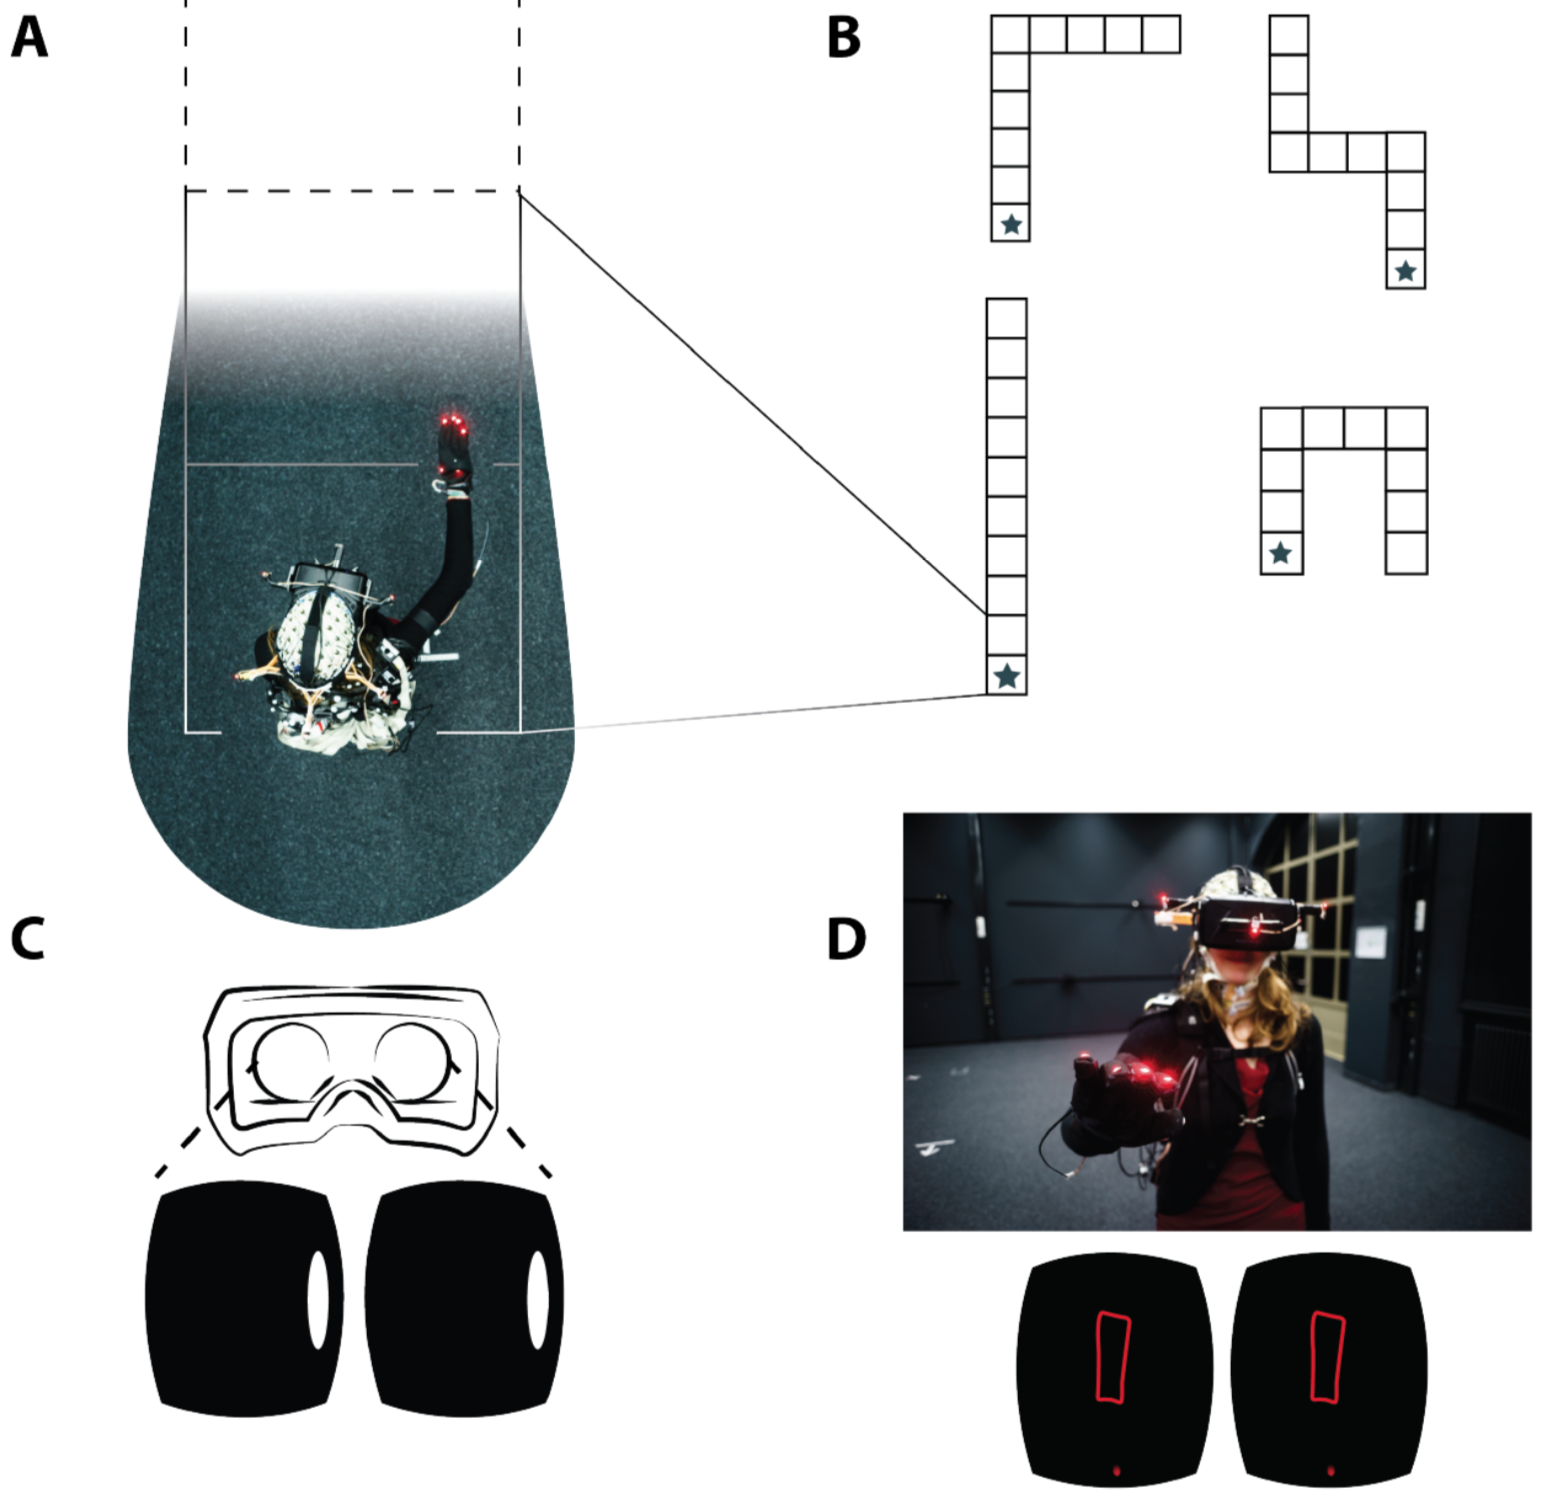
\includegraphics[width=.8\linewidth]{figures/IMT_Task.png}
\vspace{0pt}
\caption{Invisible Maze Task, \textbf{A} Participant from a bird’s eye view. \textbf{B} Participants are instructed to explore four different mazes and return to the start. \textbf{C} First-person view in binocular ""VR optics"" of a wall touch. \textbf{D} Top: Participants draw a top-down view of the explored maze. Participant is equipped with 160 channels wireless EEG, head-mounted virtual reality goggles and LEDs for motion capture. Bottom: drawn sketch map. Find a detailed description in \citep{Gehrke2018}}
\label{imt_task}
\end{figure}

% Next Paragraph: Do people behave differently in VR? And if so, does it depend on the level of experienced presence?
However, fewer studies have investigated the impact of the effectiveness of VR illusions on rich behavioral, psychometric and bio-physiological parameters. Here, the bulk of the literature focuses on (A) emotionally charged stimulus material or (B) embodiment illusions. Considering (A), \citet{Diemer2015} provide a thorough overview of the intricate interplay between presence and reactions to emotionally charged stimulation in VR. The authors observed a consistently reported link between presence and the emotional experience in VR. They argue, that by varying degrees of arousal, presence impacts psychological as well as physiological responses. Considering (B), we highlight one relevant aspect from the rich literature on the effects of full-body embodiment into avatars \citep{Maister2015}. The proteus effect characterizes behavioral perturbations depending on avatar body attributes. Yee et al. showed that participants being immersed into an 'attractive' avatar moved closer into the interpersonal space of another person \citep{Yee2007}. Further, Banakou et al. demonstrated that within participants, the sizes of objects were overestimated while embodied into a child body compared to a non-embodied baseline \citep{Banakou2013}. These examples illustrate that the level of experienced presence directly impacts mental representation of the surroundings and respectively the motor behavior.